% % steps/step01.tex
\section[گام اول: تعریف مسئله]{\faSlidersH\ \ گام اول: تعریف مسئله}
\begin{stepbox}

\field{مشکل یا نیاز اصلی چیست؟}{
    بر اساس آمارهای سازمان بهداشت جهانی (WHO) در سال ۲۰۲۲، سرطان کبد یکی از عوامل اصلی مرگ‌ومیر ناشی از سرطان در جهان به شمار می‌رود. تشخیص زودهنگام، تعیین دقیق حجم و مرزبندی تومورها نقش حیاتی در برنامه‌ریزی‌های درمانی و جراحی ایفا می‌کند. با این حال، بررسی دستی تصاویر پزشکی توسط رادیولوژیست‌ها فرآیندی بسیار زمان‌بر، خسته‌کننده و مستعد خطای انسانی (به ویژه در تفسیر مرزهای مبهم) است؛ بنابراین نیاز مبرمی به یک سیستم خودکار و دقیق وجود دارد.
}

\field{چرا بینایی ماشین برای حل آن مناسب است؟}{
    بینایی ماشین و به‌طور خاص مدل‌های یادگیری عمیق، توانایی بالایی در استخراج ویژگی‌های پیچیده و الگوهای بافتی غیرخطی از تصاویر پزشکی دارند. این سیستم‌ها می‌توانند چالش‌های سنتی پردازش تصویر در داده‌های سی‌تی اسکن (مانند کنتراست پایین بین کبد و بافت‌های نرم مجاور و همچنین تنوع شدید در شکل، اندازه و موقعیت تومورها) را با دقت و تکرارپذیری بالا حل کنند.
}

\field{هدف نهایی و خروجی مورد انتظار چیست؟}{
    هدف این پروژه، توسعه یک سیستم هوش مصنوعی مبتنی بر یادگیری عمیق جهت بخش‌بندی (\lr{Segmentation}) خودکار بافت سالم کبد و تومورهای کبدی در تصاویر \lr{CT Scan} است. خروجی مورد انتظار این سیستم، تولید ماسک‌های دقیق پیکسل‌به‌پیکسل از نواحی هدف است که عملکرد آن با معیارهای استاندارد تصویربرداری پزشکی، به ویژه ضریب شباهت دایس (\lr{Dice Similarity Coefficient - DSC}) مورد ارزیابی قرار می‌گیرد.
}

\begin{center}
    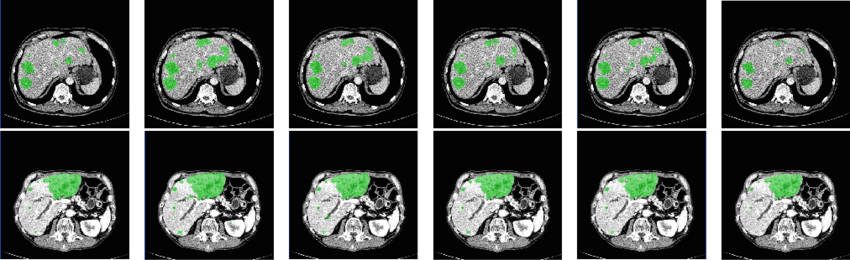
\includegraphics[width=0.85\textwidth]{images/Liver-tumor-segmentation-results-of-different-methods-on-the-LiTS-validation-dataset.png}
    \vspace{0.2cm} \\
    \footnotesize{شکل ۱ - نمونه‌ای از خروجی مورد انتظار برای بخش‌بندی تصاویر \lr{CT}. نواحی سبزرنگ نشان‌دهنده ماسک‌های مشخص‌کننده بافت کبد و تومورهای کبدی هستند.}
\end{center}



\end{stepbox}
